\section{Introduction}
Graphs are ubiquitous in various fields of life. Despite not always being explicitly identified as such, the graph data model's flexibility and simplicity make it an effective tool for modeling a diverse range of data. This includes unexpected instances, such as modeling text or images as a graph, as well as more complex instances like chemical molecules, citation networks, or connectivity encodings of the World Wide Web \cite{Mor+2020, Sca+2009}.

Although machine learning has achieved remarkable success with image classification and text generation in the last decade, the lack of a significant breakthrough in machine learning for graphs can be attributed to the graph data model's inherent flexibility and simplicity. While, for example, an image classifier constrains its input data to be a grid-like image or a text generator expects its input to be a linear sequence of words, machine learning models working on graphs cannot leverage any constraints on the format or size of their input graphs without limiting their generality. 

To put this flexibility of the graph data model into perspective and give an idea of how ubiquitous graphs are in various fields, we refer back to the examples of image classifiers and text generators and demonstrate how seemingly natural the graph data model can encode their input data. For example, images can be encoded by a graph, such that each pixel of the image corresponds to a node in the graph holding the color value, and each node is connected to its neighboring pixel nodes. Similarly, for sequential data like text files, one can encode a directed graph where each word in this file is represented as a node with the word as a feature and connected outgoingly to the next following word. For an illustrative example of the encoding idea of both cases, see \Cref{fig:example_encodings}.

In recent years, a significant amount of research has been conducted to investigate Graph Neural Networks (GNNs). The term GNN refers to any model working over graphs that utilizes neural networks (TODO: Source). Among the most promising approaches are those utilizing the message-passing architecture, which was introduced by \cite{Gil+2017} and \cite{Sca+2009}. These models are also referred to as message-passing neural networks (MPNNs) and build a subgroup of GNNs. Empirically, this framework has demonstrated strong performance across various applications \cite{Kip+2017, Ham+2017, Xu2018}. However, its expressiveness is limited, as has been proved by the works of \cite{Morris2018}, as well as \cite{Xu2018}. These works establish a connection to the commonly used Weisfeiler-Leman\footnote{Based on \href{https://www.iti.zcu.cz/wl2018/pdf/leman.pdf}{https://www.iti.zcu.cz/wl2018/pdf/leman.pdf}, we will use the spelling ``Leman'' here, as requested by A. Leman, the co-inventor of the algorithm.} algorithm (1-WL), originally proposed by \cite{Wei+1968} as a simple heuristic for the graph isomorphism problem. In particular, it has been proven that a GNN based on the message-passing architecture can, at most, be as good as the 1-WL algorithm in distinguishing non-isomorphic graphs. Furthermore, the 1-WL method demonstrates numerous similarities with the fundamental workings of the GNN architecture. It is, therefore, commonly believed that both methods are, to some extent, equivalent in their capacity to capture information in a graph.

In this work, we introduce a novel framework, which we coined ``1-WL+NN,'' which involves applying the 1-WL algorithm to an input graph and further processing the resulting information using a feedforward neural network. Thereby, we obtain a trainable framework suited for all kinds of graph-related tasks, such as graph classification, node regression, and more. In the first part of this work, we will show a theoretical equivalence between 1-WL+NN and MPNNs, such that each function computed by a 1-WL+NN can also be computed by an MPNN model and vice versa.

The interesting property of this framework compared to MPNNs and the original idea that inspired this work is the fundamental difference in how both frameworks learn and optimize themselves when applied to a specific task. Take, for example, an arbitrary classification task. While the first part of a 1-WL+NN model starts by applying the 1-WL algorithm to its input graph and retrieves a highly informative representation of this graph, the second part, the learnable feedforward network, must find common patterns in this very detailed representation that coincides with each class of the task, such that the model makes a good prediction of the actual class of its input graph. In comparison, while an MPNN is theoretically as expressive as the 1-WL algorithm, we imagine that such a model tries to find common patterns as early as possible and will drop irrelevant information as soon as possible before making a class prediction. 
Therefore, we expect a 1-WL+NN model to perform sufficiently well on its training data but poorly in generalizing for the intended task. In comparison, we expect an MPNN to generalize significantly better due to being applied directly to the input graph and being able to filter out irrelevant information.

We will use this novel framework and various empirical experiments where we compare both frameworks on multiple datasets to establish a deeper understanding of the representations learned by GNNs and try to asses reasons for better generalization abilities of GNNs.

For the ease of readability, we split this work into two parts. The first part investigates and establishes the theoretical equivalence between the frameworks of 1-WL+NN and MPNNs. In contrast, the second part deals with various experiments we conducted and discusses their empirical results.

In detail, this work starts with \Cref{sec:related_work}, where we discuss related work, milestones in GNNs over the past decade, essential properties of the 1-WL algorithm, and a subset of interesting connections between GNNs and the 1-WL algorithm. Afterward, we will start with \Cref{part1}, which begins with \Cref{sec:pre_lim}. Here, we will introduce formal definitions for both frameworks, as well as a set of notations we will use throughout the theoretical part. Afterward, in \Cref{sec:theo_connections}, we will introduce four theorems that each present a connection between both frameworks and combined prove the equivalence of both frameworks. Finally, we will prove each theorem individually after another in corresponding subsections.

The second part will deal with ...
\begin{figure}[H]
    \centering
    \begin{minipage}[b]{0.475\textwidth}
        \centering
        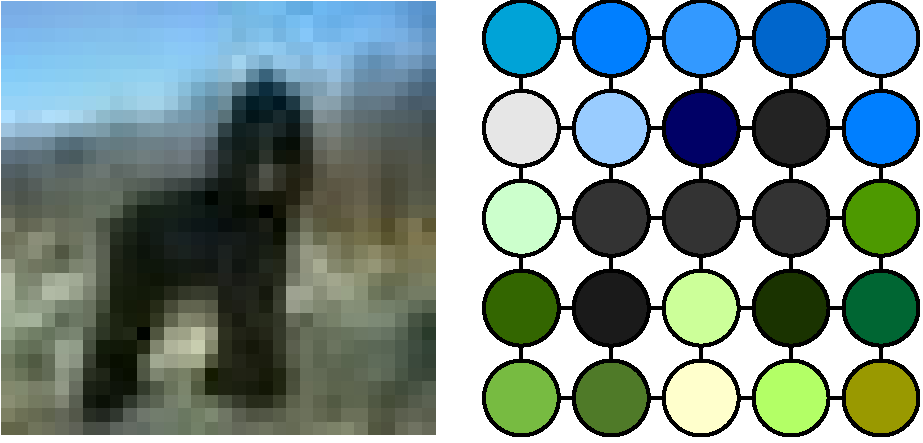
\includegraphics[width=\textwidth]{Figures/Example_Encoding_Image.pdf}
        \caption*{(a) Example for an image of a dog.\footnotemark}
    \end{minipage}
    \hfill
    \begin{minipage}[b]{0.475\textwidth}
        \centering
        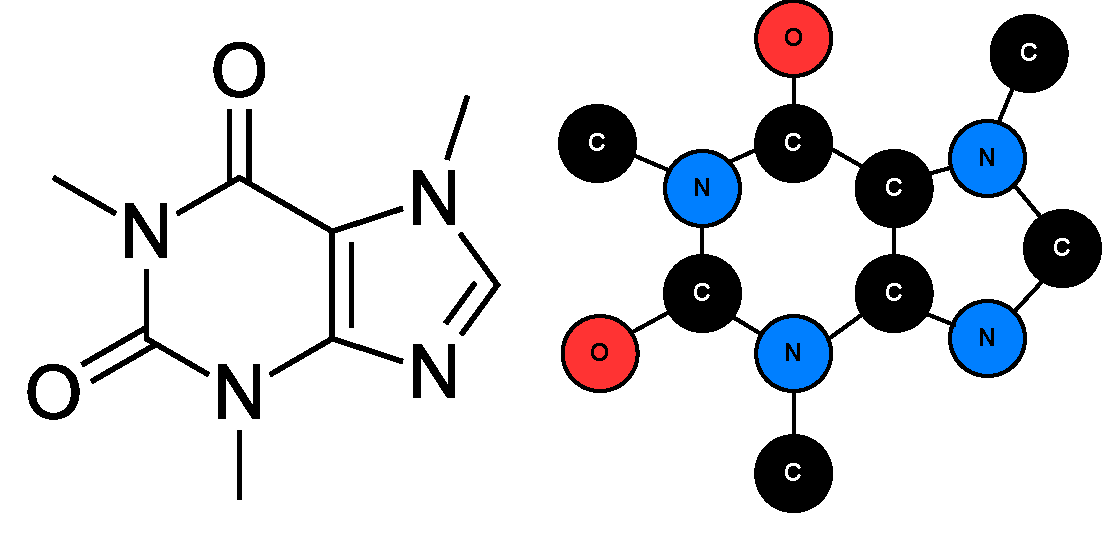
\includegraphics[width=\textwidth]{Figures/Example_Encoding_Molecule.pdf}
        \caption*{(b) Example for the molecule caffeine.}
    \end{minipage}
    \par\medskip
    \centering
    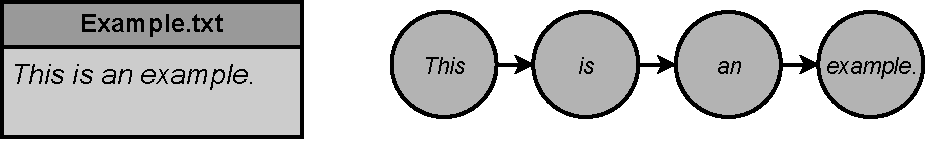
\includegraphics[scale=.5]{Figures/Example_Encoding_Text.pdf}
    \caption*{(c) Example for a text file.}
    \hfill

    \caption[Caption for LOF]{Examples of the use of graphs to encode information in a variety of domains. Note that all of these encodings are only exemplary and that in practice, encodings are typically used that capture more information than shown here.\footnotemark}
    \label{fig:example_encodings}
\end{figure}

\footnotetext[2]{The image is from the CIFAR-10 collection made available by \cite{Krizhevsky2009}.}

\footnotetext{All graphics were created using the free open source platform \href{https://www.draw.io}{https://www.draw.io}.}

\newpage